\documentclass[11pt]{article}
\usepackage{geometry}
\usepackage{booktabs}
\usepackage{hyperref}
\usepackage{graphicx}
\usepackage{subcaption}
\usepackage{tikz}
\usetikzlibrary{arrows.meta,positioning,shapes.geometric,fit,calc,decorations.pathreplacing}
\geometry{margin=1in}

\title{Agents for Temporal Grounding}
\author{Elliot Epstein}
\date{\today}

\begin{document}
\maketitle

\section{Introduction}
We propose a methodology for assigning the earliest calendar year in which a question--answer bundle could likely have been written, and apply it to produce a large, time-grounded post-training dataset based on Tulu-3.

\paragraph{Task.}
Let $x$ be a text sample. Let $P_{x,\mathrm{gt}}(t)$ denote the (latent) distribution over earliest times $t$ such that the text could be produced without relying on unavailable or speculative knowledge at time $t$, as judged by a well-informed observer. Given $x$, predict the $\alpha$-quantile of $P_{x,\mathrm{gt}}$:
\[
t_\alpha(x)
\;=\;
\inf\Bigl\{ t \;:\; \Pr_{T \sim P_{x,\mathrm{gt}}}\!\bigl(T \le t\bigr) \ge \alpha \Bigr\}.
\]

\paragraph{Interpretation.}
A fraction $\alpha$ of informed observers would judge time $t_\alpha(x)$ (or earlier) to be admissible. Times earlier than $t_\alpha(x)$ lie in the premature tail.

\paragraph{Applications.}
Synchronos LLMs are models trained on data restricted to specific year ranges. Potential applications include finance backtesting to avoid look-ahead bias, historical analysis with time-bounded knowledge, auditing model behavior under controlled knowledge cutoffs, and reproducible evaluations that fix the temporal scope of training data.

\section{Method}
Figure~\ref{fig:filtering-flow} summarizes the end-to-end pipeline. The process follows a five-step agent pipeline:
\begin{enumerate}
    \item Entity Extraction Agent: extract time-anchored entities from the question and answer bundle.
    \item Reasoner Agent: assign a best-estimate year and a 95\% confidence interval per entity.
    \item Search Query Agent: generate standalone search queries for each entity.
    \item Internet Search Agent: retrieve evidence from search results to ground the estimates.
    \item Reasoner/Synthetizer Agent: update entity confidence intervals based on the evidence and update the overall estimated year using the maximum upper bound across entities.
\end{enumerate}

\paragraph{Entity types.}
We group entities into three categories: explicit (an explicit date or event such as a product launch), implicit (a concept whose earliest admissible date could vary across observers, e.g., ``there has been a lot of discussion about global warming on the news recently''), and timeless (no time-anchored entity is present).

We do not use a database agent because there is no internal database to cross-reference in this pipeline.

\begin{figure}[t]
    \centering
    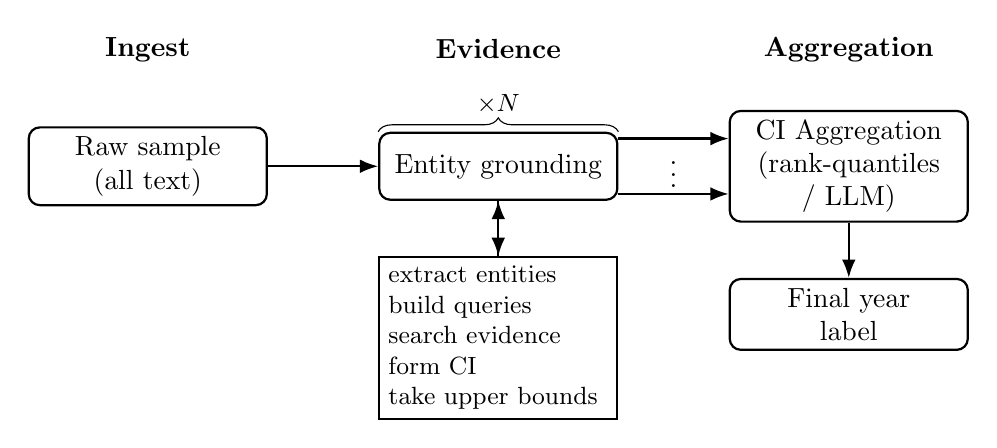
\begin{tikzpicture}[
        node distance=0.7cm and 1.0cm,
        box/.style={rectangle, rounded corners, draw=black, thick, align=center, text width=0.23\textwidth, minimum height=0.85cm},
        phase/.style={rectangle, draw=none, align=center, font=\bfseries},
        note/.style={rectangle, draw=black, thick, align=left, text width=0.23\textwidth, font=\small},
        arrow/.style={-Latex, thick}
    ]
        \node[box] (input) {Raw sample\\(all text)};
        \node[box, right=of input, xshift=0.4cm] (ground) {Entity grounding};
        \node[box, right=of ground, xshift=0.4cm] (agg) {CI Aggregation\\(rank-quantiles / LLM)};

        \node[phase, above=of input] (phase1) {Ingest};
        \path let \p1 = (phase1), \p2 = (ground) in node[phase] (phase2) at (\x2,\y1) {Evidence};
        \path let \p1 = (phase1), \p2 = (agg) in node[phase] (phase3) at (\x2,\y1) {Aggregation};

        \node[note, below=of ground] (ground_note) {extract entities\\build queries\\search evidence\\form CI\\take upper bounds};
        \node[box, below=of agg] (assign) {Final year\\label};

        \draw[arrow] (input) -- (ground);
        \draw[arrow] ([yshift=10pt]ground.east) -- ([yshift=10pt]agg.west);
        \draw[arrow] ([yshift=-10pt]ground.east) -- ([yshift=-10pt]agg.west);
        \node at ($(ground.east)!0.5!(agg.west)$) {\vdots};
        \draw[arrow] (agg) -- (assign);

        \draw[arrow] (ground) -- (ground_note);
        \draw[arrow] (ground_note) -- (ground);

        \draw[decorate, decoration={brace, amplitude=5pt}] (ground.north west) -- (ground.north east);
        \node[font=\small] at ($(ground.north)+(0,0.35)$) {$\times N$};
    \end{tikzpicture}
    \caption{Filtering pipeline for a single sample. Evidence extraction and CI aggregation are repeated for $N$ samples, then merged into a final year label.}
    \label{fig:filtering-flow}
\end{figure}

\paragraph{Annotation protocol.}
For each sample, the annotator read the question and answer, extracted relevant entities (omitting entities that are clearly older than the dominant ones), and searched to find the concept date for each entity. For each entity, we include a source link to the article stating the concept date unless the fact is trivially known. The full dev-set annotation pass took about 2 hours, or roughly 3.5 minutes per question.

\paragraph{Why not GLiNER.}
We evaluated GLiNER for entity extraction, but it is a poor fit for this task. Given fixed categories, it must both detect the entity span and map it to a category; empirically it misses entities frequently in our data. Because missed entities directly induce leakage, we instead use LLMs for the full stack (entity extraction through year estimation), with search-based evidence grounding to improve reliability.

\section{Evaluation}
\paragraph{Dev set.}
We build a 35-question dev set sampled from Tulu-3 and labeled by human annotators to design and iterate on the prompting scheme, entity grounding, and aggregation rules. We use the dev set to refine the prompting scheme and aggregation rules.

\paragraph{Test set.}
We prepared a held-out test set of 141 samples from Tulu-3, annotated by human annotators with gold years and source links in the same way as the dev set.

% \begin{table}[t]
%     \centering
%     \small
%     \begin{tabular}{lccc}
%         \toprule
%         Model & Exact acc & Conservative acc & Weighted acc \\
%         \midrule
%         \multicolumn{4}{c}{\textit{TBD}} \\
%         \bottomrule
%     \end{tabular}
%     \caption{Test-set accuracy on the 141-sample held-out evaluation set (TBD).}
%     \label{tab:filtering-test}
% \end{table}

% \begin{figure}[t]
%     \centering
%     \textit{TBD}
%     \caption{Test-set year distribution across models (TBD).}
%     \label{fig:test-year-dists}
% \end{figure}

\begin{figure}[t]
    \centering
    \includegraphics[width=1.0\textwidth]{figures/grounding_impact_test_delta_search_grid.pdf}
    \caption{Search-aided prediction error (predicted year minus ground truth) by model on the held-out test set, with negative deltas colored by failure type.}
    \label{fig:test-delta-search}
\end{figure}

\section{Results}
Key plots for this analysis are Figure~\ref{fig:grounding-conservative} and Figure~\ref{fig:grounding-delta-search}. Figure~\ref{fig:grounding-conservative} shows that search grounding improves no-leak accuracy by roughly 10 points across models, with Gemini models reaching 100\% no-leak accuracy on the dev set. Figure~\ref{fig:grounding-delta-search} shows the distribution of predicted year minus gold year; the most common failure is entity extraction, while search grounding appears reliable. We categorize error types using an LLM with access to the ground-truth answer. Figure~\ref{fig:test-delta-search} shows the search-aided prediction error (predicted year minus gold year) by model on the test set, with negative deltas colored by failure type. In many cases the difference reflects the LLM finding later references than the human annotator; this should improve once multiple annotators review each example. Without gold labels, we estimate model conservatism by counting how often each model provides the maximum year for the same prompt; Figure~\ref{fig:conservative-ensemble} summarizes these counts and two max-ensembles.

\subsection{Next Steps}
Finalize the test-set plots and tables, then:
\begin{enumerate}
    \item Measure inter-LLM consistency.
    \item Measure inter-human-rater consistency.
    \item Measure human/LLM correlation.
    \item Add a simple LLM prompting baseline.
    \item Quantify the gain from sampling $N$ times rather than 1 time.
    \item Update the test set with improved gold years once multiple annotations can be merged.
\end{enumerate}

\paragraph{Other performance metrics.}
Possible options include an asymmetric error loss averaged over samples,
$L = \max(0, -e) + \beta \cdot \max(0, e)$ where $e = \hat{y} - y$,
$\hat{y}$ is the predicted year, and $y$ is the gold year. This penalizes
underestimates more than overestimates when $\beta < 1$, but it is harder to
interpret and requires choosing $\beta$. Another option is an equally weighted
average of exact year match and no-leak accuracy, which is easy to interpret but
does not distinguish between off-by-one errors and large errors.

\begin{figure}[t]
    \centering
    \includegraphics[width=0.9\textwidth]{figures/grounding_impact_conservative.pdf}
    \caption{No-leak accuracy (predicted year $\ge$ gold) before vs.\ after search grounding.}
    \label{fig:grounding-conservative}
\end{figure}

\begin{figure}[t]
    \centering
    \includegraphics[width=1.0\textwidth]{figures/grounding_impact_delta_search_grid.pdf}
    \caption{Search-aided prediction error (predicted year minus ground truth) by model, with negative deltas colored by failure type.}
    \label{fig:grounding-delta-search}
\end{figure}

\begin{figure}[t]
    \centering
    \includegraphics[width=0.9\textwidth]{figures/conservatism_counts_max_combo.pdf}
    \caption{Most-conservative counts over 50 questions, with max-ensembles of Gemini 3 Flash + GPT-5-mini and Gemini 3 Pro + GPT-5.2 (ties count).}
    \label{fig:conservative-ensemble}
\end{figure}

\clearpage
\section{Discussion}
Two observations stand out: Gemini 3 Flash performs better than Gemini 3 Pro, and GPT-5-mini is similar to GPT-5.2. It would be valuable to explore whether this stems from smaller models producing more conservative intervals and from the asymmetric risk profile that penalizes underestimates more than overestimates.

\section{Data Filtering}
We label each supervised (SFT), preference, and RLVR sample with the minimum calendar year consistent with its question--answer bundle; the prompt structure is detailed in Appendix~A. We considered deterministic filtering, but it was difficult to capture all edge cases with a rule-based approach. The latest sweep (session \texttt{2026-01-06\_14-10PT}) processed 30{,}549 SFT examples, 29{,}510 preference examples, and three RLVR datasets (7{,}358 GSM, 7{,}372 MATH, 14{,}958 IFEval) with a conservative policy that uses the most recent referenced year. Figures~\ref{fig:sft}--\ref{fig:rlvr} show year and category distributions for each dataset family and validate cutoff integrity.

\begin{figure}[t]
    \centering
    \begin{subfigure}{0.48\textwidth}
        \centering
        \includegraphics[width=\linewidth]{figures/year_shards_allenai-tulu-3-sft-mixture_2026-01-06_22-10Z_n49948_year_histogram.pdf}
        \caption{Year distribution (SFT).}
    \end{subfigure}
    \hfill
    \begin{subfigure}{0.48\textwidth}
        \centering
        \includegraphics[width=\linewidth]{figures/year_shards_allenai-tulu-3-sft-mixture_2026-01-06_22-10Z_n49948_category_histogram.pdf}
        \caption{Category distribution (SFT).}
    \end{subfigure}
    \caption{Filtering summary for the TÜLU-3 SFT mixture (session \texttt{2026-01-06\_14-10PT}, $n=30{,}549$).}
    \label{fig:sft}
\end{figure}

\begin{figure}[t]
    \centering
    \begin{subfigure}{0.48\textwidth}
        \centering
        \includegraphics[width=\linewidth]{figures/year_shards_allenai-llama-3-1-tulu-3-8b-preference-mixture_2026-01-06_22-10Z_n50000_year_histogram.pdf}
        \caption{Year distribution (DPO).}
    \end{subfigure}
    \hfill
    \begin{subfigure}{0.48\textwidth}
        \centering
        \includegraphics[width=\linewidth]{figures/year_shards_allenai-llama-3-1-tulu-3-8b-preference-mixture_2026-01-06_22-10Z_n50000_category_histogram.pdf}
        \caption{Category distribution (DPO).}
    \end{subfigure}
    \caption{Filtering summary for the TÜLU-3 preference mixture (session \texttt{2026-01-06\_14-10PT}, $n=29{,}510$).}
    \label{fig:dpo}
\end{figure}

\begin{figure}[t]
    \centering
    \begin{subfigure}{0.48\textwidth}
        \centering
        \includegraphics[width=\linewidth]{figures/year_shards_allenai-rlvr-gsm_2026-01-06_22-10Z_n7473_year_histogram.pdf}
        \caption{Year distribution (RLVR-GSM).}
    \end{subfigure}
    \hfill
    \begin{subfigure}{0.48\textwidth}
        \centering
        \includegraphics[width=\linewidth]{figures/year_shards_allenai-rlvr-gsm_2026-01-06_22-10Z_n7473_category_histogram.pdf}
        \caption{Category distribution (RLVR-GSM).}
    \end{subfigure}

    \begin{subfigure}{0.48\textwidth}
        \centering
        \includegraphics[width=\linewidth]{figures/year_shards_allenai-rlvr-math_2026-01-06_22-10Z_n7500_year_histogram.pdf}
        \caption{Year distribution (RLVR-MATH).}
    \end{subfigure}
    \hfill
    \begin{subfigure}{0.48\textwidth}
        \centering
        \includegraphics[width=\linewidth]{figures/year_shards_allenai-rlvr-math_2026-01-06_22-10Z_n7500_category_histogram.pdf}
        \caption{Category distribution (RLVR-MATH).}
    \end{subfigure}

    \begin{subfigure}{0.48\textwidth}
        \centering
        \includegraphics[width=\linewidth]{figures/year_shards_allenai-rlvr-ifeval_2026-01-06_22-10Z_n14973_year_histogram.pdf}
        \caption{Year distribution (RLVR-IFeval).}
    \end{subfigure}
    \hfill
    \begin{subfigure}{0.48\textwidth}
        \centering
        \includegraphics[width=\linewidth]{figures/year_shards_allenai-rlvr-ifeval_2026-01-06_22-10Z_n14973_category_histogram.pdf}
        \caption{Category distribution (RLVR-IFeval).}
    \end{subfigure}
    \caption{Filtering summary for the RLVR datasets (session \texttt{2026-01-06\_14-10PT}, GSM $n=7{,}358$, MATH $n=7{,}372$, IFEval $n=14{,}958$).}
    \label{fig:rlvr}
\end{figure}

\clearpage
\appendix
\section{Model Training on Filtered Data}
\subsection{SFT setup}
We fine-tune Qwen3-4B-Base with LoRA adapters on the 2007-capped TÜLU-3 SFT subset (26{,}431 examples) with a 4,096-token context length. Training runs for two epochs with linear decay, short warmup, and small per-device batches with gradient accumulation. Tokens per second per GPU are around 1{,}000. The LoRA run takes about 3 hours 2 minutes for 300M tokens (padding included). LoRA uses roughly 45 GB of GPU memory; full fine-tuning is about 10$\times$ slower, and TÜLU-2 showed lower LoRA performance.

\begin{table}[t]
    \centering
    \begin{tabular}{ll}
        \toprule
        Component & Setting \\
        \midrule
        Base model & Qwen3-4B-Base \\
        Tokenizer & Qwen3-4B-Base tokenizer \\
        Training data & TÜLU-3 SFT, year \(\le\) 2007 (26{,}431 examples) \\
        Sequence length & 4{,}096 tokens \\
        Batch size & 1 sample per device \\
        Gradient accumulation & 16 steps (effective 16 samples per device) \\
        Optimizer schedule & Linear decay with 3\% warmup \\
        Learning rate & \(1 \times 10^{-4}\) \\
        Weight decay & 0.0 \\
        Epochs & 2 \\
        LoRA configuration & rank 64, \(\alpha=16\), dropout 0.1 \\
        Memory optimizations & Flash attention and gradient checkpointing \\
        Checkpoint cadence & Every 500 steps (keep last 3) \\
        \bottomrule
    \end{tabular}
    \caption{Supervised fine-tuning configuration for the LoRA run.}
    \label{tab:sft-lora}
\end{table}

\begin{figure}[t]
    \centering
    \includegraphics[width=\textwidth]{figures/lora_ft_metrics.png}
    \caption{LoRA SFT training metrics: disk utilization (GB), reserved GPU memory (GB), learning rate, total tokens, per-device tokens per second, and train loss.}
    \label{fig:lora-metrics}
\end{figure}

\paragraph{Hardware.}
All runs use three NVIDIA RTX A6000 GPUs (48 GB each). The LoRA configuration fits within a single A6000 with limited headroom for data loading and logging.

\subsection{SFT results}
We run the TÜLU-3 dev evaluation suite with \texttt{run\_tulu3\_dev\_limit100.sh}, dispatching 11 suites and limiting each task to 100 examples (MMLU uses 100 questions per subject, totaling 5{,}700 evaluations). This gives a fast signal across reasoning, coding, alignment, and factuality. Task summaries: GSM8K (grade-school math word problems), DROP (reading comprehension with numeric reasoning), Minerva Math (competition math problems across seven domains), HumanEval/HumanEval+ (Python coding pass@10), IFEval (instruction-following), PopQA (entity-centric factual QA), MMLU (multiple-choice knowledge across 57 subjects), AlpacaEval v2 (pairwise preference wins), BBH (hard reasoning tasks with CoT), TruthfulQA (robustness to falsehoods).

Table~\ref{tab:tulu} summarizes the latest snapshot for Qwen3-4B-Base and placeholder columns for +SFT, +DPO, and +RLVR checkpoints (marked ``--''). The SFT evaluation is still running; partial results are shown where available. Scores are percentages, with \texttt{n} denoting evaluated examples.

\begin{table}[t]
    \centering
    \begin{tabular}{llcccccc}
        \toprule
        Task & Metric & Qwen3-4B Base & +SFT & +DPO & +RLVR & $n$ \\
        \midrule
        GSM8K & Exact match & 83.00 & 83.00 & -- & -- & 100 \\
        DROP & F1 & 52.15 & 57.16 & -- & -- & 100 \\
        Minerva Math (avg) & Exact match & 39.14 & -- & -- & -- & 700 \\
        HumanEval & pass@10 & 95.84 & 97.30 & -- & -- & 100 \\
        HumanEval+ & pass@10 & 94.80 & 93.28 & -- & -- & 100 \\
        IFEval & Prompt loose acc & 40.00 & 43.00 & -- & -- & 100 \\
        PopQA & Accuracy & 17.00 & 20.00 & -- & -- & 100 \\
        MMLU (mc) & Macro accuracy & 74.46 & 74.44 & -- & -- & 5{,}700 \\
        AlpacaEval v2 & Len-ctrl win rate & 6.54 & -- & -- & -- & 100 \\
        BBH (cot-v1) & Macro accuracy & -- & -- & -- & -- & -- \\
        TruthfulQA & MC2 & 54.48 & 45.59 & -- & -- & 100 \\
        \bottomrule
    \end{tabular}
    \caption{Primary metrics for the TÜLU-3 dev suite (Qwen3-4B-Base, 100-example subsets). The BBH run is still executing at this scale; results will be inserted once the evaluation completes.}
    \label{tab:tulu}
\end{table}

\paragraph{Filtering Cost.}
The current filtering pass uses GPT-5-mini with batch requests at \$0.25/\$2.00 per 1M input/output tokens; the batch discount halves these rates to \$0.125/\$1.00. Table~\ref{tab:filtering-costs} summarizes per-sample token averages, current costs, and projections for the full SFT/preference corpus plus the RLVR targets. TÜLU-3 still requires filtering 900k SFT examples and 250k preference examples beyond the current subset; projected costs scale linearly with per-sample token counts. For prompts under 200k tokens, Gemini 3 Flash is priced at \$0.50/\$3.00 per 1M input/output tokens (similar to GPT-5-mini), while Gemini 3 Pro is \$2.00/\$12.00 (similar to GPT-5.2).

\begin{table}[t]
    \centering
    \small
    \resizebox{\textwidth}{!}{%
    \begin{tabular}{lrrrrrrr}
        \toprule
        Dataset & Current $n$ & Tokens/sample & Current cost & Projected $n$ & GPT-5-mini & GPT-5.2 & GPT-5.2 Pro \\
        \midrule
        SFT & 30{,}549 & 1{,}661 & \$20.46 & 930{,}549 & \$623 & \$4.36k & \$52.3k \\
        Preference & 29{,}510 & 2{,}437 & \$25.08 & 279{,}510 & \$238 & \$1.66k & \$20.0k \\
        RLVR GSM & 7{,}358 & 2{,}167 & \$6.78 & 8{,}790 & \$8.10 & \$56.7 & \$680 \\
        RLVR MATH & 7{,}372 & 1{,}653 & \$3.68 & 7{,}500 & \$3.74 & \$26.2 & \$315 \\
        RLVR IFEval & 14{,}958 & 1{,}690 & \$10.81 & 15{,}000 & \$10.84 & \$75.9 & \$910 \\
        \bottomrule
    \end{tabular}
    }
    \caption{Filtering costs (USD) under batch pricing. Projected counts use 900k/250k additional SFT/preference samples and RLVR targets of 8.79k (GSM), 7.5k (MATH), and 15k (IFeval).}
    \label{tab:filtering-costs}
\end{table}

Downstream, we select shards with a year-bounded loader to enforce knowledge cutoffs (e.g., 2014).

\clearpage
\appendix
\section{SFT Filtering Prompt}
\begin{verbatim}
You label the minimum calendar year (between 2001 and 2025) required to answer
a question without temporal leakage. The label must never precede any fact
mentioned in the sample; when uncertain, err toward the later year so that no
future knowledge sneaks into earlier buckets.

You receive a dataset-specific question plus an answer bundle (which may contain
multiple sections).
These are supervised instruction-tuning pairs: treat the question as the user
prompt and the response as the assistant answer.
Pick the smallest year Y in [2001, 2025] so that a model with knowledge through
year Y could answer confidently, considering EVERYTHING in both the question and
the answer bundle. If no specific time-dependent knowledge is required, output
2001.

Rules:
- Identify all time-anchored entities in the question and answer bundle.
- For each entity, provide a best_estimate year plus a 95% confidence interval.
- Use the entity's founding/release/announcement year (not the future target year).
- Set overall "year" to the maximum upper bound across all entity confidence intervals.
- If a range is mentioned (e.g., "released between 2008 and 2015"), use that as
  the entity's interval.
- If information is older than 2001, still respond with 2001.
- Do not hallucinate years; use only dates grounded in the text or well-known facts.
- Additionally, assign the question to one category from this list:
  general_knowledge, math, coding, science, history, law, finance, health,
  creative_writing, multi_lingual, instruction_following, reasoning, other.

You may reason internally, but the final output must be a single JSON object only.
Do not include any extra text or code fences.

Return JSON with these required fields and meanings:
- "year": integer in [2001, 2025] for the minimum safe year.
- "confidence": "low" | "medium" | "high".
- "category": one of the allowed categories listed above.
- "justification": short reason for the chosen year.
- "entities": object mapping entity names to an object with:
  - "best_estimate": best estimate year for founding/release/announcement.
  - "confidence_interval_95": [yearA, yearB] containing the best estimate; yearA/yearB
    can be the same.
  - "search_query": a standalone query to verify the year estimate.
- If no entities are found, use an empty object for "entities".

Illustrative example (output only):
{"year": 2006, "confidence": "high", "category": "general_knowledge",
"justification": "Answer references tweets, a concept only available after
Twitter launched in 2006, so 2006 is the earliest safe year.",
"entities": {"tweet": {"best_estimate": 2006, "confidence_interval_95": [2006, 2006],
"search_query": "When was Twitter launched?"}}}

<question>
{sample.question}
</question>
<answer_bundle>
{sample.answer}
</answer_bundle>
Return JSON exactly in this schema:
{"year": 2001, "confidence": "low|medium|high",
"category": "one of the allowed categories",
"justification": "why year is required",
"entities": {"entityA": {"best_estimate": 2008, "confidence_interval_95": [2007, 2009],
"search_query": "When was entityA released?"},
"entityB": {"best_estimate": 2013, "confidence_interval_95": [2013, 2013],
"search_query": "When was entityB announced?"}}}
\end{verbatim}

\paragraph{SFT Mixture Data.}
The TÜLU 3 SFT mixture used for training contains 939{,}344 samples from the sources below.

\begin{table}[t]
    \centering
    \small
    \begin{tabular}{lrl}
        \toprule
        Dataset & Prompts & License \\
        \midrule
        CoCoNot & 10{,}983 & ODC-BY-1.0 \\
        FLAN v2 (ai2-adapt-dev/flan\_v2\_converted) & 89{,}982 & -- \\
        No Robots & 9{,}500 & CC-BY-NC-4.0 \\
        OpenAssistant Guanaco & 7{,}132 & Apache 2.0 \\
        Tulu 3 Persona MATH & 149{,}960 & ODC-BY-1.0 \\
        Tulu 3 Persona GSM & 49{,}980 & ODC-BY-1.0 \\
        Tulu 3 Persona Python & 34{,}999 & ODC-BY-1.0 \\
        Tulu 3 Persona Algebra & 20{,}000 & ODC-BY-1.0 \\
        Tulu 3 Persona IF & 29{,}980 & ODC-BY-1.0 \\
        NuminaMath-TIR & 64{,}312 & Apache 2.0 \\
        Tulu 3 WildGuardMix & 50{,}000 & Apache 2.0 \\
        Tulu 3 WildJailbreak & 50{,}000 & ODC-BY-1.0 \\
        Tulu 3 Hardcoded & 240 & CC-BY-4.0 \\
        Aya & 100{,}000 & Apache 2.0 \\
        WildChat GPT-4 & 100{,}000 & ODC-BY-1.0 \\
        TableGPT & 5{,}000 & MIT \\
        SciRIFF & 10{,}000 & ODC-BY-1.0 \\
        Evol CodeAlpaca & 107{,}276 & Apache 2.0 \\
        \bottomrule
    \end{tabular}
    \caption{TÜLU 3 SFT mixture composition. Source details: Brahman et al. (2024), Longpre et al. (2023), Rajani et al. (2023), Kopf et al. (2024), Beeching et al. (2024), Han et al. (2024), Wildteaming (2024), Singh et al. (2024), Zhao et al. (2024), Zha et al. (2023), Wadden et al. (2024), Luo et al. (2023).}
    \label{tab:sft-mixture}
\end{table}

\end{document}
